\documentclass{article}

% ── NeurIPS 2026 style ───────────────────────────────────────────────────────
% Options: [preprint] for arXiv, [final] for camera-ready, default = anonymous
\usepackage[preprint]{neurips_2026}

% ── Additional packages (not loaded by the sty) ──────────────────────────────
\usepackage{amsmath,amssymb}
\usepackage{booktabs}
\usepackage{xcolor}
\usepackage{graphicx}
\usepackage{microtype}
\usepackage{enumitem}
\usepackage[colorlinks=true,linkcolor=blue!60!black,citecolor=green!50!black,
            urlcolor=blue!60!black]{hyperref}
\graphicspath{{figures/}}

% ── Title ────────────────────────────────────────────────────────────────────
\title{The Completion Fallacy in LLM Evaluation:\\A Process-Sensitive Probe for Cumulative State Tracking Predicts Agent Performance Beyond Task Completion}

\author{%
  Dengzhe Hou\textsuperscript{1,\dag}\hspace{1.5em}
  Lingyu Jiang\textsuperscript{1}\hspace{1.5em}
  Deng Li\textsuperscript{2}\hspace{1.5em}
  Zirui Li\textsuperscript{1}\\[2pt]
  \bf Fangzhou Lin\textsuperscript{1,3,4}\hspace{1.5em}
  Michael Zielewski\textsuperscript{1}\hspace{1.5em}
  Kazunori D Yamada\textsuperscript{1}\\[6pt]
  \normalfont\textsuperscript{1}Tohoku University\hspace{1em}
  \textsuperscript{2}Lappeenranta-Lahti University of Technology LUT\\[1pt]
  \textsuperscript{3}Texas A\&M University\hspace{1em}
  \textsuperscript{4}Worcester Polytechnic Institute\\[2pt]
  {\small \texttt{hou.dengzhe.t8@dc.tohoku.ac.jp}}\\[1pt]
  {\small \textsuperscript{\dag}Corresponding author.}
}

\date{}

\begin{document}

\maketitle

% ─────────────────────────────────────────────────────────────────────────────
\begin{abstract}
LLM benchmarks overwhelmingly measure task completion but not how the
model processes information---a gap we call the
\emph{Completion Fallacy}. We propose the Cognitive Evaluation
Framework (CEF), a \emph{provisional} research agenda of process-sensitive
behavioral probes grounded in cognitive science, and report a
construct-development pilot for one probe family, WMF-AM
(cumulative arithmetic state tracking under load), as an existence
proof that process-sensitive measurement adds value beyond completion.

In a 20-model open-weight pilot (13 families, 0.5B--35B parameters),
WMF-AM significantly predicts performance on a deterministic 10-task
multi-step agent battery ($\tau{=}0.612$, $p{<}0.001$) and this
signal persists after partialling out completion
($\tau_{\text{partial}}{=}0.411$, $p{=}0.011$): a process probe
captures downstream-relevant variance that a 100-item completion
battery misses, surviving all four confound controls including a
joint partial for completion and model scale.
CEF's four-dimension structure is an unvalidated working taxonomy;
WMF-AM is the sole thoroughly piloted sub-dimension, and
generalization to cloud API models and robustness-oriented downstream
tasks remains open.
\end{abstract}

% ─────────────────────────────────────────────────────────────────────────────
\section{Introduction}
\label{sec:intro}

Current evaluation measures the products of cognition, not cognition
itself. Benchmarks such as HotpotQA~\citep{yang2018hotpotqa},
MMLU~\citep{hendrycks2021mmlu}, and AgentBench~\citep{liu2023agentbench}
tell us what LLMs accomplish, not \emph{how} they process
information. We call this the \emph{Completion Fallacy}: the inference that
task-completion success alone is sufficient for inferring latent
process competence. Completion metrics are often useful for outcome
prediction, but completion alone does not distinguish agents that are
reliable under distribution shift and process-coherent from those
that are not---a special case of
Goodhart's law~\citep{goodhart1984,manheim2018categorizing}.

Several recent results converge on this point.
PAE~\citep{xie2026m3} finds 27--78\% of agent successes involve
corrupted trajectories; Fragile
Thoughts~\citep{aravindan2026fragile} and Robust Answers Fragile
Logic~\citep{jiang2026robustanswersfragilelogic} show correct answers
produced despite broken reasoning chains;
Turpin et al.~\citep{turpin2023language} demonstrate unfaithful
chain-of-thought explanations. These are instances of multiple
realizability~\citep{putnam1967}: identical outcomes produced by
categorically different processes---a pattern also documented as
underspecification~\citep{damour2022underspecification} and shortcut
learning~\citep{geirhos2020shortcut}.

This paper is a \emph{position paper with a pilot study}: we make a conceptual argument (Completion Fallacy), propose a provisional organizing framework (CEF), and provide empirical existence-proof evidence for one specific probe (WMF-AM). CEF's four-dimension structure is unvalidated; our evidence speaks to one sub-dimension.

This paper makes three contributions.
\textbf{(1)~Formalization.} We characterize the Completion Fallacy
(Section~\ref{sec:fallacy}) and identify three structural failure modes
of outcome-only evaluation: one empirically illustrated (diagnostic blindness,
with quantified model-pair evidence) and two hypothesized (uninformative
failure diagnosis, safety blindness), each requiring further empirical confirmation.
\textbf{(2)~Framework and pilot.} We propose the Cognitive Evaluation
Framework (CEF, Section~\ref{sec:cef}), a \emph{provisional, unvalidated
research agenda} organized around four cognitive-science dimensions.
A 20-model study
(Section~\ref{sec:pilot}) provides existence-proof evidence that
WMF-AM---a probe of \emph{cumulative arithmetic state tracking under
load}---captures process variance invisible to completion
and predicts performance on a deterministic 10-task multi-step
agent battery beyond completion ($\tau{=}0.612$, $p{<}0.001$;
partial $\tau{=}0.411$, $p{=}0.011$), including for non-state-tracking tasks ($\tau{=}0.623$).
\textbf{(3)~Protocols.} We provide complete experimental protocols
for all 11 CEF sub-dimensions as a community resource
(Appendix~\ref{app:protocols}).
A glossary of all acronyms appears in Table~\ref{tab:glossary}
(Appendix~\ref{app:glossary}).

\paragraph{Three separable claims.}
(a)~The \emph{general thesis}: completion metrics alone are insufficient
for inferring process quality. This claim is supported by converging
independent evidence (PAE, Fragile Thoughts, Turpin et al.) and does
not depend on CEF.
(b)~\emph{CEF as one proposed framework}: a taxonomy of
process-sensitive probes organized around cognitive science. Other
frameworks are possible; CEF is offered as a concrete research agenda.
(c)~\emph{WMF-AM as one operationalization}: the pilot provides
existence-proof evidence for (a) through one specific probe family.
The completion-fallacy claim does not rise or fall with any single
sub-benchmark.

\textbf{Evidence map.} WMF-AM has multi-seed, multi-template,
yoked-control, and downstream predictive validity evidence
(\emph{study-supported}); EMC-lite, MCC-MA, and CLA-CR have single-seed
evidence (\emph{preliminary}); remaining sub-dimensions have protocols only
(\emph{proposed}).
Table~\ref{tab:valstatus} in Appendix~\ref{app:tables} gives the full
development status. Section~\ref{sec:fallacy} formalizes the thesis;
Section~\ref{sec:cef} presents the CEF taxonomy;
Section~\ref{sec:pilot} reports the WMF-AM pilot;
Section~\ref{sec:discussion} discusses limitations and implications.

% ─────────────────────────────────────────────────────────────────────────────
\section{The Completion Fallacy and Related Work}
\label{sec:fallacy}

\paragraph{Three failure modes (one empirically illustrated, two hypothesized).}
\textbf{(F1) Diagnostic blindness} \emph{[empirically illustrated]}: models
with near-identical completion scores can have very different process profiles.
In the pilot study: 30/105 model pairs with $|\Delta\text{completion}| \leq 0.05$
show $|\Delta\text{WMF-AM}| \geq 0.10$ (exploratory; threshold-dependent---at
$\leq 0.03 / \geq 0.15$, 18/105 pairs qualify). WMF-AM spans 0.050--0.983 among
20 models while completion spans only 0.44--0.92; among mid-to-large models
($\geq$3B), completion SD $= 0.052$ versus WMF-AM SD $= 0.228$.
\textbf{(F2) Uninformative failure diagnosis} \emph{[hypothesized]}: current
benchmarks report \emph{that} an agent failed, not \emph{why}---whether the
bottleneck is state tracking, metacognitive calibration, or episodic confusion.
Process-sensitive profiles, if validated at scale, could in principle decompose
failure into actionable sub-dimensions. This function of CEF awaits full validation.
\textbf{(F3) Safety blindness} \emph{[hypothesized]}: pattern-matching agents
(which fail predictably at distribution shift) are indistinguishable from genuine
reasoners on standard benchmarks. Whether WMF-AM or other process probes predict
this failure mode remains an open empirical question requiring dedicated robustness study.

\paragraph{Empirical support.}
Multiple realizability is empirically the norm in frontier LLMs.
Fragile Thoughts~\citep{aravindan2026fragile} and Robust Answers
Fragile Logic~\citep{jiang2026robustanswersfragilelogic} provide direct
evidence: correct answers are regularly produced despite corrupted
reasoning steps. Turpin et al.~\citep{turpin2023language} show
chain-of-thought explanations can be systematically unfaithful;
Lanham et al.~\citep{lanham2023measuring} measure this faithfulness
gap directly. Uesato et al.~\citep{uesato2022solving} demonstrate that
process-based feedback outperforms outcome-based feedback for
mathematical reasoning. PAE~\citep{xie2026m3} extends this to agent
trajectories, finding 27--78\% of successful completions involve
corrupted intermediate actions. These are Agent B/C behaviors at scale.

\paragraph{From outcome underdetermination to process probes.}
Outcome metrics cannot distinguish process quality. Three questions
follow: (a)~What can task success not identify? Whether behavior
generalizes under shift, whether confidence reflects error detection,
or whether memory discriminates episodes.
(b)~Which gaps require process evidence versus robustness or adversarial
testing? Process probes are needed when the question is \emph{how} the
model processes information.
(c)~Why CEF? Robustness testing~\citep{ribeiro2020checklist} addresses
perturbation; trace audits~\citep{turpin2023language,lanham2023measuring}
address reasoning-to-output coupling; adversarial evaluations address
worst-case performance. CEF targets the space left uncovered:
parametrically controlled, cognitively grounded probes of process quality
under multi-turn load.

\paragraph{Positioning.}
Cognitive science has developed rigorous measurement paradigms for each
function CEF addresses: working memory capacity~\citep{miller1956,baddeley1974},
metacognitive monitoring/control~\citep{flavell1979,nelson1990},
episodic memory~\citep{tulving1972episodic,johnson1993}, and cognitive
load adaptation~\citep{sweller1988,miyake2000}. CEF adapts their
measurement logic for API-level LLM evaluation. This does not require
LLMs to have human cognition; it requires that the constructs pick out
capabilities that matter for deployment.
NeuroCognition~\citep{haznitrama2026neuropsychologicallygroundedevaluationllm}
measures cognitive \emph{ability}; CEF measures \emph{process quality}
under load. Strong Memory, Weak
Control~\citep{de2025strong} studies executive function in isolated
tasks; CEF tests the same constructs under sustained interference.
Entity Tracking~\citep{entitytracking2023} is prior art for WMF-AM;
Intelligence Degradation~\citep{wang2026intelligence} is prior art for
CLA. Bowman and Dahl~\citep{bowman2021fix} argue benchmarking requires
construct-level validity; CheckList~\citep{ribeiro2020checklist}
introduced behavioral testing templates; CEF extends both.
\emph{Process supervision}~\citep{lightman2023verify,uesato2022solving}
trains models using step-level labels; CEF \emph{measures} process
quality but does not prescribe training signals.
\emph{Mechanistic interpretability} analyzes internal representations;
CEF operates at the API level (prompt/response only) and is
complementary: interpretability explains \emph{why} a process score is
low, while CEF identifies \emph{that} it is low.
A full related-work table appears in Appendix~\ref{app:related}.

\paragraph{Formal definitions.}
Let $Y_i \in [0,1]$ denote the outcome score and $Z_i \in [0,1]$ a
process-sensitive measure for model $i$, both defined relative to a
specific benchmark suite and model population. We say outcome metrics
are \emph{statistically insufficient with respect to a downstream criterion $D$} if
process measures provide significant incremental prediction of $D$
beyond completion: partial $\tau(Z, D \mid Y) > 0$ at conventional
$\alpha$. This is a \emph{benchmark-conditional} claim---it asserts
insufficiency for a given $\langle Y, Z, D \rangle$ triple, not a
universal property. Statistical insufficiency does not by itself
determine practical or deployment relevance: the latter depends on
whether the incremental signal is large enough and the criterion
important enough to warrant the additional measurement cost.
In the study, partial $\tau(\text{WMF-AM},
\text{Agent} \mid Y) = 0.411$ ($p = 0.011$, $N{=}20$), meeting this
criterion. The completion--process correlation ($\tau_{\text{WMF-AM, completion}}{=}0.279$,
$p{=}0.150$, $N{=}15$, bootstrap 95\% CI $[-0.156, 0.637]$) is
suggestive of divergence but not confirmed at this sample size.
\emph{Falsification}: CEF's core claim would be undermined if, across
multiple probe families and downstream criteria, process measures
never provided significant incremental prediction beyond completion.
The four-dimension structure is a working taxonomy;
dimensional separability requires factor analysis at $N \geq 30$.


% ─────────────────────────────────────────────────────────────────────────────
\section{The Cognitive Evaluation Framework (CEF)}
\label{sec:cef}

CEF is a \emph{hypothesis-generating taxonomy}---an organizational
framework for process-sensitive probes, not an empirically validated
instrument. We emphasize this hierarchy explicitly: the paper
presents \emph{one thoroughly piloted probe family} (WMF-AM) as a
concrete existence proof, embedded within a broader speculative
taxonomy (CEF) that offers candidate dimensions for future
investigation. The taxonomy should be read as a research agenda, not
as a validated instrument. Only WMF-AM has multi-evidence pilot support
(predictive validity, seed reliability, template stability, yoked
control, arithmetic-vs-assignment ablation, paraphrase stability);
three sub-dimensions have preliminary single-seed results; the
remainder are protocol-only (Appendix~\ref{app:tables},
Table~\ref{tab:valstatus}).
The taxonomy is offered to organize future research; the number and
boundaries of dimensions are working hypotheses pending factor analysis
at $N \geq 30$.
A full glossary of acronyms (WMF, MCC, EMC, CLA, and their
sub-dimension suffixes) appears in Table~\ref{tab:glossary}
(Appendix~\ref{app:glossary}).

\begin{figure}[t]
\centering
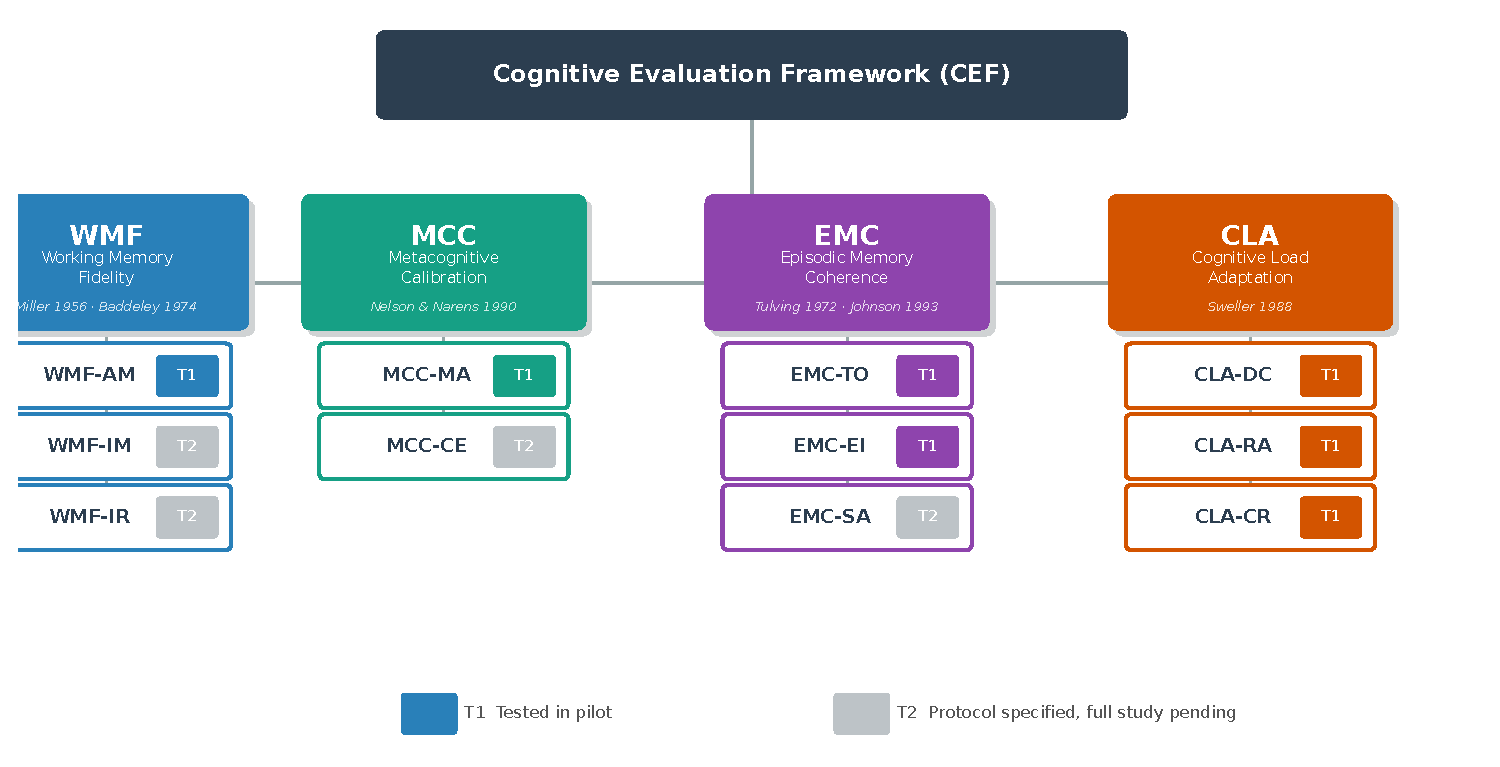
\includegraphics[width=\textwidth]{fig3_framework.pdf}
\caption{\textbf{CEF architecture.} Four dimensions (WMF, MCC, EMC, CLA)
derived from cognitive science, decomposed into 11 proposed
sub-dimensions. \textbf{Solid border}: pilot-supported (WMF-AM).
\textbf{Dashed border}: preliminary or proposed probes awaiting the
$N \geq 15$ study.}
\label{fig:framework}
\end{figure}

\paragraph{Design principles.}
Each dimension must have (i)~a cognitive science anchor---an established
measurement paradigm with validated human operationalizations,
(ii)~a documented evaluation gap not covered by existing benchmarks,
and (iii)~API-level testability requiring only prompt/response access.
We use labels like ``working memory'' as \emph{operational shorthand}
for behavioral probes, not as claims about LLM mechanisms.
``WMF-AM'' means accuracy on sequential state-tracking tasks degrades
with depth $K$; it does not mean LLMs have a working memory buffer
(see Appendix~\ref{app:labels} for full discussion).

\paragraph{Four dimensions.}
Table~\ref{tab:dims} summarizes each dimension's target capacity,
canonical failure signature, and exclusions.

\begin{table}[t]
\centering
\small
\caption{CEF dimensions: target, failure signature, and exclusions.
Detailed sub-dimension definitions appear in Appendix~\ref{app:subdims}.}
\label{tab:dims}
\resizebox{\linewidth}{!}{%
\begin{tabular}{lp{3cm}p{3cm}p{3cm}}
\toprule
\textbf{Dim} & \textbf{Target} & \textbf{Failure signature} & \textbf{Excluded} \\
\midrule
WMF & Active maintenance and transformation of state under load
  & Accuracy drops as concurrent items exceed threshold
  & Long-context retrieval; knowledge recall \\
MCC & Self-monitoring of errors (MA) and correction of flagged errors (CE)
  & Confident-wrong; flagging without correction
  & General calibration (ECE); cross-model detection \\
EMC & Temporal ordering, cross-episode discrimination, source attribution
  & Episode blending; source misattribution
  & Single-turn retrieval; semantic memory \\
CLA & Degradation shape and resource scaling under load
  & Cliff-edge failure; non-recovery
  & Knowledge difficulty; unrelated complexity \\
\bottomrule
\end{tabular}}
\end{table}

\paragraph{Flagship probe: WMF-AM.}
WMF-AM (Active Manipulation) is a probe of \textbf{cumulative arithmetic
state tracking under load}, inspired by working-memory span paradigms.
An initial numeric state is presented, $K$ sequential additive/subtractive
operations arrive, and the model must report the final cumulative state.
The pilot uses depths $K \in \{3,5,7\}$ (dissociation study) and $K
\in \{2,4,6,8,12\}$ (yoked cancellation control), across three surface
forms (points scoring, warehouse inventory, bank accounts). Prior entity
tracking~\citep{entitytracking2023} tests passive retrieval; WMF-AM
tests \emph{sequential arithmetic transformation} under load.
\emph{Scope of the construct}: WMF-AM specifically measures difficulty
with maintaining a running cumulative sum across $K$ additive/subtractive
operations. It does not claim to measure general working-memory capacity,
and it may partially reflect standalone arithmetic competence;
a completed last-operation-only ($K{=}1$) control addresses this:
13/15 models achieve near-ceiling single-step arithmetic accuracy
($\bar{x}{=}0.957$) versus $\bar{x}{=}0.151$ at $K{=}7$,
indicating that cumulative accumulation under load—not arithmetic
skill per se—is the primary difficulty driver.

\textbf{Worked example ($K{=}3$, points form):} \emph{``Alice starts
with 10 points. Alice gains 5 points. Alice loses 3 points. Alice gains
7 points. What is Alice's current score?''} Correct answer: 19.
Scoring: exact match (1 if the model outputs 19, 0 otherwise).
A model that tracks each update cumulatively
($10 \to 15 \to 12 \to 19$) succeeds; a model that performs only the
last operation or guesses a plausible number fails. At $K{=}7$, the
chain length taxes state maintenance, producing the diagnostic
depth$\times$accuracy interaction.
\textbf{Yoked control example ($K{=}3$):} \emph{``Alice starts with 10
points. Alice gains 5 points. Alice loses 5 points. Alice gains 3
points. Alice loses 3 points. Alice gains 7 points. Alice loses 7
points. What is Alice's current score?''} Correct answer: 10 (initial
state). Each operation is immediately followed by its inverse, requiring
identical arithmetic but no cumulative tracking.

\paragraph{MCC: Metacognitive Calibration.}
MCC decomposes metacognition into monitoring accuracy (MCC-MA: predict
which of 20 answers are wrong; Pearson $r$) and control efficacy
(MCC-CE: flag uncertain answers, then revise them; decomposed into
flagging rate, correction efficacy, and false alarm
rate)---Reflexion~\citep{shinn2023reflexion} conflates these. Unlike
Gnosis~\citep{ghasemabadi2025can} (requires internals), MCC-MA uses
prompting under multi-turn load. The 2$\times$2 taxonomy
(Table~\ref{tab:mcc}) makes the decomposition actionable: each cell
implies a different architectural intervention.

\begin{table}[t]
\centering
\small
\caption{Metacognitive profile taxonomy. Each cell implies a different
intervention target.}
\label{tab:mcc}
\resizebox{\linewidth}{!}{%
\begin{tabular}{lcc}
\toprule
& \textbf{High MCC-CE} & \textbf{Low MCC-CE} \\
\midrule
\textbf{High MCC-MA} & Genuine metacognition & Monitoring works; correction broken \\
\textbf{Low MCC-MA} & Correction works; detection unreliable & No metacognitive capability \\
\bottomrule
\end{tabular}}
\end{table}

\paragraph{EMC: Episodic Memory Coherence.}
EMC tests temporal ordering (EMC-TO), cross-episode discrimination
(EMC-EI), and source attribution (EMC-SA) under interference. Current
benchmarks measure binary retrieval; no protocol tests whether a model
situates retrieved facts in time and context. The EMC-lite pilot
(Section~\ref{sec:pilot}) covers a related but narrower slice.

\paragraph{CLA: Cognitive Load Adaptation.}
CLA characterizes the \emph{shape} of the performance-versus-load
function. CLA-DC (degradation curve smoothness) correlates highly with
WMF-AM ($\tau = 0.905$) in the original 7-model set. We \emph{provisionally
collapse} CLA-DC onto WMF: both involve state tracking under load.
Factor analysis with $N{=}15$ models is planned to determine whether
this collapse holds. This does not invalidate the taxonomy---it
refines it.
CLA-RA (resource allocation) and CLA-CR (capacity recovery after
high-load block) are structurally independent and cannot collapse onto
WMF-AM by design (they measure recovery, not degradation).
Intelligence Degradation~\citep{wang2026intelligence} reports
\emph{that} performance drops; CLA characterizes \emph{how}.
Full definitions, composites, and scoring rules are in
Appendix~\ref{app:subdims}; Table~\ref{tab:ataglance} in
Appendix~\ref{app:tables} summarizes all 11 sub-dimensions.

\paragraph{Construct validity framework.}
Following Cronbach and Meehl~\citep{cronbach1955construct},
Messick~\citep{messick1989validity}, Campbell and
Fiske~\citep{campbell1959convergent}, and Jacobs and
Wallach~\citep{jacobs2021measurement}, each dimension requires convergent
validity (correlation with independent process-sensitive measures) and
divergent validity (low correlation with completion). The study supports
divergent validity for WMF-AM ($\tau = 0.279$ with a 100-item
completion battery, $N{=}15$; bootstrap 95\% CI $[-0.156, 0.637]$)
and cross-template rank stability ($\tau_{\text{bare,chat}} = 0.524$,
$p = 0.006$). CEF would
be falsified if all dimensions collapsed onto a single factor
indistinguishable from task completion.
Appendix~\ref{app:falsify} provides full construct-to-probe mapping
with confounds and falsification criteria for each pilot-tested probe.

% ─────────────────────────────────────────────────────────────────────────────
\section{Pilot Study: Process-Sensitive Differentiation}
\label{sec:pilot}

\paragraph{Statistical methodology.}
All rank correlations use Kendall's $\tau$-b (accounts for ties).
Partial $\tau$ uses Somers residualization:
\[
  \tau_{XY|Z} \;=\; \frac{\tau_{XY} - \tau_{XZ}\,\tau_{YZ}}
  {\sqrt{(1-\tau_{XZ}^2)(1-\tau_{YZ}^2)}}.
\]
Bootstrap 95\% CIs: 10{,}000 nonparametric model-level resamples
(percentile method). Permutation tests: 100{,}000 permutations.
All $p$-values are two-sided. The two pre-specified confirmatory
analyses are predictive validity ($\tau = 0.612$) and template stability
($\tau = 0.524$); both survive Bonferroni correction at
$\alpha = 0.025$. All other correlations are exploratory.

\begin{table}[h]
\centering
\small
\caption{\textbf{Key analyses at a glance.} All $\tau$ = Kendall's $\tau$-b.
C = confirmatory (pre-specified, Bonferroni-corrected); E = exploratory.}
\label{tab:keyanalyses}
\resizebox{\linewidth}{!}{%
\begin{tabular}{@{}lp{3.2cm}ccccl@{}}
\toprule
\textbf{Relation} & \textbf{Subset} & $\tau$ & $N$ & $p$ & \textbf{95\% CI} & \textbf{Type} \\
\midrule
WMF-AM $\to$ Agent overall & All models & 0.612 & 20 & $<$0.001 & $[0.360, 0.814]$ & C \\
Bare $\leftrightarrow$ Chat template ranks & 15 models & 0.524 & 15 & 0.006 & --- & C \\
WMF-AM $\to$ Agent (partial $|$ completion) & All models & 0.411 & 20 & 0.011 & --- & E \\
WMF-AM $\to$ Agent (partial $|$ $\log$ params) & All models & 0.503 & 20 & $<$0.01 & --- & E \\
WMF-AM $\to$ Agent (partial $|$ compl.\ $+$ $\log$ params) & All models & 0.389 & 20 & 0.016 & --- & E \\
WMF-AM $\to$ Agent non-WMF (7 tasks) & All models & 0.623 & 20 & $<$0.001 & --- & E \\
WMF-AM $\to$ Agent WMF-heavy (3 tasks) & All models & 0.527 & 20 & 0.003 & --- & E \\
WMF-AM $\leftrightarrow$ completion & 15 models & 0.279 & 15 & 0.150 & $[-0.156, 0.637]$ & E \\
CONV-RFPOC $\leftrightarrow$ AGENT-PQ & 7 models & 0.905 & 7 & 0.003 & --- & E \\
\bottomrule
\end{tabular}}
\end{table}

\emph{Note on sample sizes.} Different analyses use different subsets:
$N{=}20$ for all predictive validity and completion-battery analyses
(the full study set); $N{=}15$ for WMF-AM template stability and
divergent validity (original 7 + expansion 8; before small models
were added); $N{=}7$ for convergent validity only (original models
with AGENT-PQ and CONV-RFPOC data collected). All sample sizes are
reported explicitly at each result.

{\sloppy
Twenty open-weight models from thirteen architectural families form the
study set: seven original models (Qwen 7B/14B/32B, Llama 3.1:8b,
Gemma 2:27b, DeepSeek-R1:14b, Mistral:7b), eight expansion models
(Phi-3:14b, Gemma-2:9b, Qwen-2.5:3b, Llama-3.2:3b, DeepSeek-R1:7b,
Mixtral:8x7b, Command-R:35b, Yi:34b), and five small baseline models
(0.5B--2B parameters; Table~\ref{tab:pilot}).
\par}
Models were evaluated in six phases. Phase~1 (Outcome Correctness)
used a 100-item battery spanning five domains (factual, math, science,
reasoning, language) at five difficulty levels, temperature $= 0$.
Phase~2 (WMF-AM) administered 15 probes at depths $K \in \{3,5,7\}$
with 4 independent random seeds for all 20 models.
Phase~3 (MCC-MA) applied a 20-problem self-monitoring probe.
Phase~4 (Yoked Cancellation Control) administered 20 trials per depth at
$K \in \{2,4,6,8,12\}$ using operations that cancel (gain then lose,
transfer then reverse), so the correct answer equals the initial state
despite requiring identical arithmetic parsing as WMF-AM.
Phase~5 (Template Harmonization) re-administered WMF-AM under three
prompt wrappers (bare, chat, chain-of-thought) to test sensitivity to
surface format.
Phase~6 (Agent Validation) administered 10 multi-step agent tasks
(tool use, multi-step reasoning, state tracking) to all 20 models
to test predictive validity.
All models are Ollama-hosted open-weight variants using default chat
templates, fp16 quantization where available, and greedy decoding
(temperature $= 0$, no top-$p$ sampling). No task overlap exists
between phases (full study matrix in Appendix~\ref{app:studymatrix}).
Table~\ref{tab:methods} summarizes the experimental design.

\begin{table}[t]
\centering
\small
\caption{\textbf{Study design summary.} All phases: temperature $= 0$,
greedy decoding, Ollama-hosted models with default chat templates.
All 20 models evaluated with 4 seeds for WMF-AM.}
\label{tab:methods}
\resizebox{\linewidth}{!}{%
\begin{tabular}{@{}llcccl@{}}
\toprule
\textbf{Phase} & \textbf{Probe} & \textbf{Depths} & \textbf{Items} & \textbf{Seeds} & \textbf{Scoring} \\
\midrule
1.\ Outcome & 100-item battery (5 domains) & --- & 100 & 1 & Exact match (0/1) \\
2.\ WMF-AM & State tracking & $K{=}3,5,7$ & 15/depth & 4 & Exact match on final state \\
3.\ MCC-MA & Self-monitoring & --- & 20 & 1 & Pearson $r$ (predicted vs actual) \\
4.\ Yoked & Cancellation ops & $K{=}2,4,6,8,12$ & 20/depth & 1 & Exact match on initial state \\
5.\ Template & 3 prompt wrappers & $K{=}3,5,7$ & 15/depth & 1 & Rank stability ($\tau$) \\
6.\ Agent & 10 multi-step tasks & --- & 10 & 1 & Process quality (0--1) \\
\bottomrule
\end{tabular}}
\end{table}

\begin{figure}[t]
\centering
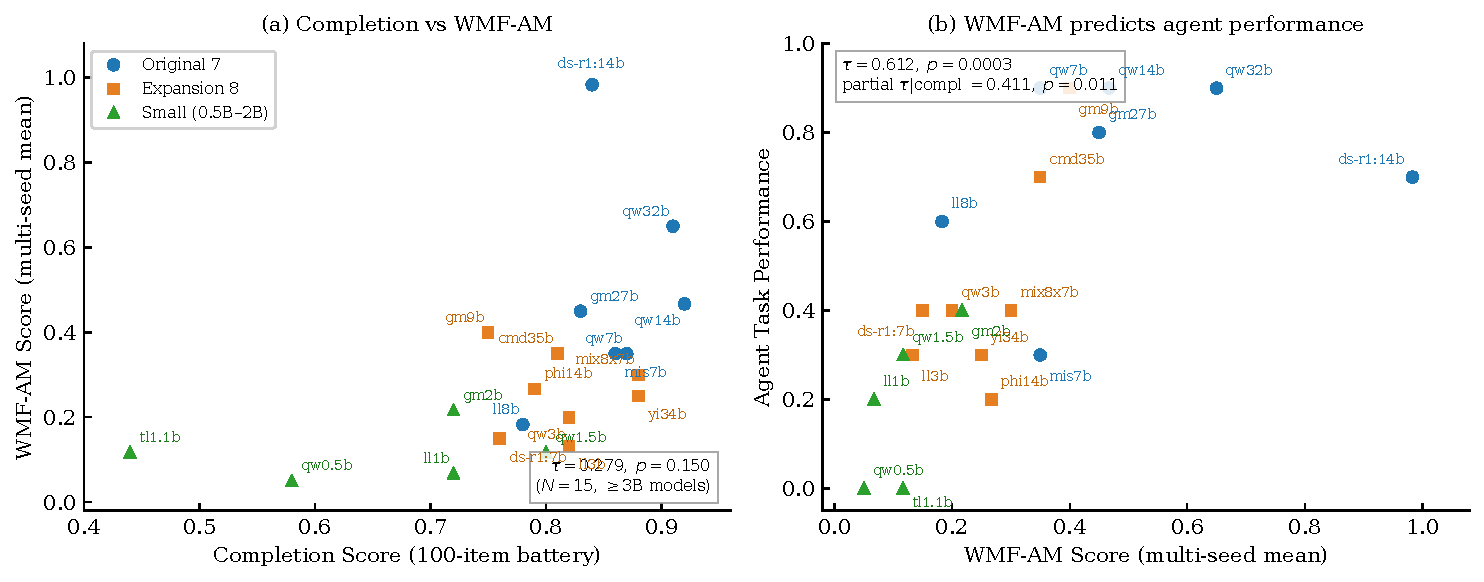
\includegraphics[width=\textwidth]{fig1_dissociation.pdf}
\caption{\textbf{(a)} Completion clusters while WMF-AM spans a wide range
($N{=}20$, 13 families). \textbf{(b)} WMF-AM predicts downstream agent
performance ($\tau{=}0.612$, $p{<}0.001$) even after controlling for
completion (partial $\tau{=}0.411$, $p{=}0.011$).
Blue circles = original 7; orange squares = expansion 8; green triangles = small models (0.5B--2B).}
\label{fig:dissociation}
\end{figure}

\paragraph{Main result: process measures provide incremental prediction beyond completion on a multi-step agent battery.}
Figure~\ref{fig:dissociation} and Table~\ref{tab:pilot} present the key
finding across $N{=}20$ models from 13 families. WMF-AM (4-seed means)
spans 0.050--0.983 ($\Delta = 0.933$) while the 100-item completion
battery spans 0.44--0.92 ($\Delta = 0.480$).
Among the 15 mid-to-large models ($\geq$3B), completion clusters
at 0.75--0.92 (SD $= 0.052$) while WMF-AM spans 0.133--0.983 (SD $= 0.228$):
completion masks substantial process-quality differences.
\textbf{Predictive validity (scoped claim):} WMF-AM significantly predicts
performance on a deterministic 10-task multi-step agent battery
($\tau = 0.612$, $p < 0.001$, $N{=}20$;
bootstrap 95\% CI $[0.360, 0.814]$). Crucially, this relationship
holds after partialling out completion: partial $\tau = 0.411$
($p = 0.011$), demonstrating that WMF-AM captures information about
downstream capability \emph{beyond} what completion provides.
Completion also predicts agent performance ($\tau = 0.428$, $p = 0.012$),
but WMF-AM provides \emph{incremental} prediction.
The primary evidence is threefold: (1)~significant predictive validity,
(2)~significant template stability ($\tau = 0.524$, $p = 0.006$), and
(3)~WMF-AM reliably differentiates models in a dimension
that completion does not fully capture.

\begin{table}[t]
\centering
\small
\resizebox{\linewidth}{!}{%
\begin{tabular}{llccccc}
\toprule
Model & Family & Outcome & WMF-AM & Agent & Yoked & WMF$-$Yoked \\
\midrule
\multicolumn{7}{l}{\emph{Original 7 (all 4-seed WMF-AM)}} \\
deepseek-r1:14b & DeepSeek & 0.840 & \textbf{0.983} & 0.70 & 0.810 & $+$0.173 \\
qwen2.5:32b     & Qwen     & 0.910 & 0.650 & \textbf{0.90} & 1.000 & $-$0.350 \\
qwen2.5:14b     & Qwen     & 0.920 & 0.467 & \textbf{0.90} & 0.710 & $-$0.243 \\
gemma2:27b      & Gemma    & 0.830 & 0.450 & 0.80 & 0.620 & $-$0.170 \\
qwen2.5:7b      & Qwen     & 0.870 & 0.350 & \textbf{0.90} & 0.770 & $-$0.420 \\
mistral:7b      & Mistral  & 0.860 & 0.350 & 0.30 & 0.550 & $-$0.200 \\
llama3.1:8b     & Llama    & 0.780 & 0.183 & 0.60 & 0.340 & $-$0.157 \\
\midrule
\multicolumn{7}{l}{\emph{Expansion 8 (all 4-seed WMF-AM)}} \\
gemma2:9b       & Gemma    & 0.750 & 0.400 & \textbf{0.90} & 0.960 & $-$0.560 \\
command-r:35b   & Cohere   & 0.810 & 0.350 & 0.70 & 0.920 & $-$0.570 \\
mixtral:8x7b    & Mistral  & 0.880 & 0.300 & 0.40 & 1.000 & $-$0.700 \\
phi3:14b        & Phi      & 0.790 & 0.267 & 0.20 & 0.950 & $-$0.683 \\
yi:34b          & Yi       & 0.880 & 0.250 & 0.30 & 1.000 & $-$0.750 \\
qwen2.5:3b      & Qwen     & 0.820 & 0.200 & 0.40 & 0.970 & $-$0.770 \\
deepseek-r1:7b  & DeepSeek & 0.760 & 0.150 & 0.40 & 0.940 & $-$0.790 \\
llama3.2:3b     & Llama    & 0.820 & 0.133 & 0.30 & 0.510 & $-$0.377 \\
\midrule
\multicolumn{7}{l}{\emph{Small models (broader baseline)}} \\
gemma2:2b       & Gemma    & 0.720 & 0.217 & 0.40 & --- & --- \\
qwen2.5:1.5b    & Qwen     & 0.800 & 0.117 & 0.30 & --- & --- \\
tinyllama:1.1b  & TinyLlama& 0.440 & 0.117 & 0.00 & --- & --- \\
llama3.2:1b     & Llama    & 0.720 & 0.067 & 0.20 & --- & --- \\
qwen2.5:0.5b    & Qwen     & 0.580 & 0.050 & 0.00 & --- & --- \\
\midrule
$\Delta$ & — & 0.480 & \textbf{0.933} & 0.90 & — & — \\
\bottomrule
\end{tabular}}
\caption{\textbf{Pilot study ($N{=}20$, 13 families).}
Outcome = 100-item battery; WMF-AM = 4-seed mean; Agent = multi-step
task performance (10 tasks). WMF-AM predicts agent performance
($\tau = 0.612$, $p < 0.001$) even after controlling for completion
(partial $\tau = 0.411$, $p = 0.011$). Yoked column shows
cancellation-control accuracy (original 15 only).}
\label{tab:pilot}
\end{table}

\paragraph{Completion battery design and broader baseline.}
Phase~1 uses a 100-item battery spanning five domains (factual, math,
science, reasoning, language) at five difficulty levels, yielding score
resolution of 0.01. With the addition of 5 small models (0.5B--2B),
scores now range from 0.44 (tinyllama:1.1b) to 0.92 (qwen2.5:14b)
(SD $= 0.131$, $N{=}20$), a substantial improvement over the original
15-model range of 0.75--0.92 (SD $= 0.052$). The broader range
strengthens interpretation: completion now correlates with agent performance
($\tau = 0.428$, $p = 0.012$), but WMF-AM provides significant
\emph{incremental} prediction (partial $\tau = 0.411$, $p = 0.011$).
Among the 15 mid-to-large models ($\geq$3B), the outcome range remains
compressed (SD $= 0.052$), confirming that range restriction is a
property of the model population, not the battery design. Difficulty-level
analysis confirms the battery discriminates
(level-5 items: 0.0--1.0 spread; level-1 items: 0.73--0.95).

\paragraph{Exploratory architectural observations.}
Reasoning-specialized architecture (deepseek-r1:14b, $0.983$)
outperforms general-purpose models despite similar parameter counts.
Scaling within families yields modest gradients (Qwen 3B$\to$32B:
$0.311 \to 0.650$). The yoked control reveals an important confound
decomposition: only deepseek-r1:14b shows positive WMF$-$Yoked
residual ($+0.173$), suggesting it alone achieves genuine cumulative
state tracking beyond per-operation parsing. All other models show
negative residuals, with the largest gaps in smaller models
(deepseek-r1:7b: $-0.829$).
Figure~\ref{fig:depth} shows the depth-dependent
degradation curves for all 15 models.

\paragraph{Alternative explanations and template sensitivity.}
WMF-AM scores may reflect nuisance factors beyond state tracking:
instruction-following ability, tokenizer effects on numeric parsing,
scratchpad/chain-of-thought policy differences, or prompt-format
sensitivity. Phase~5 (template harmonization) directly tests the last
concern: across 15 models $\times$ 3 templates, model rankings under
bare and chat wrappers are significantly correlated
($\tau_{\text{bare,chat}} = 0.524$, $p = 0.006$), indicating that
WMF-AM rankings are moderately robust to surface-format variation.
Chain-of-thought (CoT) templates push nearly all models to ceiling
($\geq 0.93$), eliminating variance.

\textbf{Target construct clarification:} WMF-AM is designed to measure
\emph{default state-tracking capability under a fixed prompt regime}
(no scratchpad, no chain-of-thought). It deliberately probes the
model's internalized processing rather than its externalized reasoning
when given scaffolding. The CoT ceiling effect is therefore not a
validity threat but a \emph{construct boundary}: WMF-AM measures what
the model can do without externalized reasoning
aids~\citep{nye2021show}, which is the relevant capability for
deployment contexts where intermediate outputs are not monitored. The moderate bare$\leftrightarrow$chat stability
($\tau = 0.524$, not near 1.0) indicates some prompt sensitivity
remains; this is a known limitation.
The yoked control isolates arithmetic parsing, but instruction-following
and tokenizer effects remain live confounds.
\textbf{Ablation results ($N{=}15$):}
\emph{(i)~Non-arithmetic state tracking}
(3 domains~$\times$~$K\in\{3,5,7\}$, 10 problems each):
when operations involve direct-assignment updates (color
``Alice's color changes to blue'', location, status) instead of
numeric accumulation, models achieve near-ceiling accuracy
(mean $0.98$, range $0.91$--$1.00$), versus the WMF-AM arithmetic
range of $0.20$--$0.72$.
Direct-assignment tracking is solved by remembering the most recent
value per entity; arithmetic tracking requires maintaining a
\emph{running cumulative sum} across $K$ additive/subtractive
operations---a strictly harder representational demand.
The floor--ceiling contrast confirms that WMF-AM difficulty is
driven by \emph{arithmetic accumulation} under load,
not generic entity-state tracking.
This does not rule out that WMF-AM partially reflects standalone
arithmetic skill; a completed last-operation-only ($K{=}1$) control
addresses this: 13/15 models achieve near-ceiling single-step
arithmetic accuracy (mean $0.957$) yet floor at $K{=}7$ accumulation
(mean $0.151$), ruling out single-step arithmetic as the primary
difficulty driver. Broader multi-step serial-composition alternatives
(e.g., error propagation, sequential prompt processing) cannot be
excluded without further mechanistic analysis.
\emph{(ii)~Prompt paraphrase}
(5 templates: original, formal, casual, minimal, verbose):
model rankings are stable across natural-language rephrasings;
mean cross-template Kendall~$\tau = 0.54$ ($5/6$ pairs $p < 0.05$);
original-vs-formal $\tau = 0.857$ ($p < 0.001$).
The stripped ``minimal'' template induces task failure rather than rank
reversal, consistent with insufficient-context degradation rather
than construct invalidity.
Rankings on the paraphrase-original template correlate
near-perfectly with the main WMF-AM results:
$\tau = 0.951$ ($p = 0.004$, $N{=}7$ overlapping models).
\emph{(iii)~Completed in prior loops:} three surface forms (points,
inventory, accounts), three prompt wrappers (bare, chat, CoT),
and four random seeds---all showing stable inter-model rank orderings.

\begin{figure}[t]
\centering
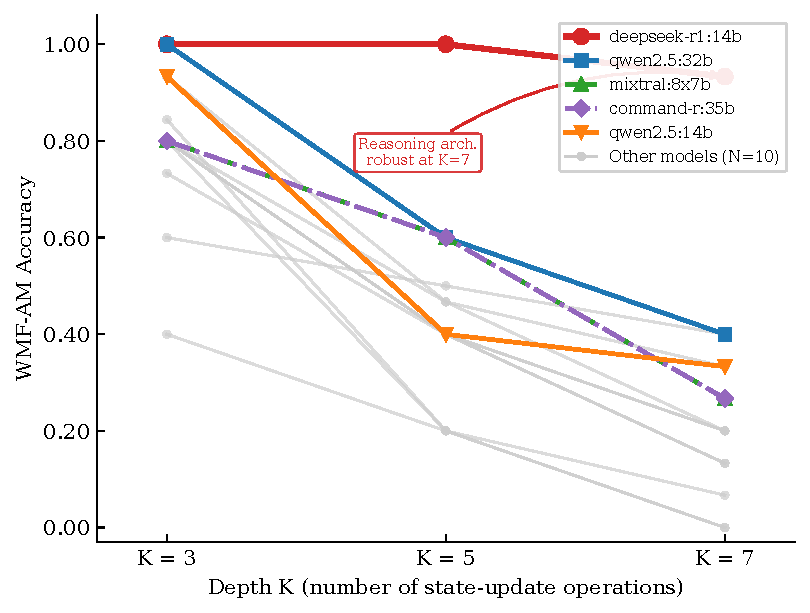
\includegraphics[width=0.72\textwidth]{fig2_depth_profile.pdf}
\caption{\textbf{WMF-AM accuracy by depth $K$ ($N{=}15$, chat template).}
deepseek-r1:14b (red) maintains near-perfect accuracy; all others
degrade sharply at $K \geq 5$. Top 5 models highlighted.}
\label{fig:depth}
\end{figure}

\paragraph{Predictive validity: agent task performance.}
Phase~6 administered 10 multi-step agent tasks (3 requiring tool use
with state tracking, 3 multi-step reasoning chains, 2 general
problem-solving, 2 constrained planning) to all 20 models.
Each task is scored 0--1 by \emph{deterministic verification}: intermediate
and final states are checked against ground-truth answers via exact
match (no LLM judge). This yields the \textbf{Agent score} used in
all predictive validity analyses. (A separate LLM-judged process quality
metric, AGENT-PQ, is available for the original 7 models only and used
solely in convergent validity; see Appendix~\ref{app:agentpq}.)
Agent scores range from 0.00
(qwen2.5:0.5b, tinyllama:1.1b) to 0.90 (qwen2.5:14b/32b/7b, gemma2:9b).

WMF-AM significantly predicts agent performance: $\tau = 0.612$
($p < 0.001$, $N{=}20$; bootstrap 95\% CI $[0.360, 0.814]$);
Table~\ref{tab:keyanalyses} summarizes all confirmatory and exploratory
correlations at a glance.
\textbf{Confound controls} (all surviving with $p < 0.02$):
(i)~partial $\tau$ controlling for completion score: $0.411$ ($p = 0.011$);
(ii)~partial $\tau$ controlling for $\log(\text{parameter count})$:
$0.503$ ($p < 0.01$, exploratory)---the relationship is not driven by model scale;
(iii)~joint partial $\tau$ controlling for \emph{both} simultaneously:
$0.389$ ($p = 0.016$, exploratory)---WMF-AM retains significant
incremental signal after accounting for both outcome performance and
model size jointly;
(iv)~within-family analysis (Qwen, $N{=}6$, 0.5B--32B):
$\tau = 0.894$ ($p = 0.016$), showing the relationship holds
\emph{within} a single architecture family.
\textbf{Criterion contamination control (pre-registered split):}
To rule out the most direct objection---that WMF-AM predicts the agent
battery merely because both involve state tracking---we split the 10
tasks into WMF-heavy (3 tool-use tasks explicitly requiring sequential
state tracking: inventory management, multi-step booking, resource allocation)
and non-WMF (7 tasks: multi-step reasoning, planning,
general problem-solving, constrained optimization---none require sequential
cumulative state tracking).
WMF-AM predicts \emph{non-WMF tasks more strongly}
($\tau = 0.623$, $p < 0.001$) than WMF-heavy tasks
($\tau = 0.527$, $p = 0.003$), arguing against the simplest
criterion-overlap explanation. Shared latent demands (sequential
execution discipline, multistep consistency) cannot be fully excluded,
but the split result undermines the most direct contamination account.
\textbf{Leave-one-out robustness:} removing any single model, the
WMF-AM $\to$ agent $\tau$ ranges $[0.537, 0.624]$ (mean $0.582$)---no
single model drives the effect.
\textbf{Scope:} these results demonstrate incremental predictive signal
beyond completion and scale in this sample of open-weight models.
Generalization to cloud API models and robustness under distribution
shift remain open questions.

\paragraph{Yoked cancellation control.}
To isolate active state tracking from per-operation arithmetic parsing,
we designed a stricter control: each operation is immediately followed
by its inverse (``Alice gains 3 points'' then ``Alice loses 3 points''),
so the correct answer always equals the initial state despite requiring
identical arithmetic processing as WMF-AM. This eliminates the shortcut
in the original inert control (where the answer was trivially the
initial state without any computation).

\textbf{Result:} Table~\ref{tab:pilot} (Yoked column) shows that most
models achieve high yoked-control accuracy (0.51--1.00) but substantially
\emph{lower} WMF-AM accuracy, indicating the WMF-AM difficulty is
genuine cumulative state tracking beyond arithmetic parsing.
The corrected residual (WMF$-$Yoked) is negative for 14/15 models,
meaning per-operation parsing inflates raw WMF-AM scores.
With the 100-item completion battery,
$\tau(\text{WMF}{-}\text{Yoked},\;\text{Outcome}) = 0.125$
($p = 0.519$, $N{=}15$) and raw WMF-AM $\tau = 0.279$ ($p = 0.150$):
neither the raw nor the residual score significantly predicts outcome
quality, strengthening the independence claim. The near-universal
negative WMF$-$Yoked residuals (14/15 models) confirm that
per-operation arithmetic parsing substantially inflates raw WMF-AM
scores, and the yoked control successfully decomposes WMF-AM into a
state-tracking component and an arithmetic-parsing confound.

\paragraph{Measurement robustness.}
Multi-seed reliability: all 15 models evaluated with 4 independent seeds
$\times$ 15 probes. Expansion-model SDs range 0.073--0.144 (mean 0.108),
comparable to original-model variability. Cross-template stability:
$\tau_{\text{bare,chat}} = 0.524$ ($p = 0.006$); $\tau_{\text{chat,cot}}
= 0.314$ ($p = 0.114$). See Appendix~\ref{app:robustness} for full
analyses.

\paragraph{Complementary probes (preliminary; see Appendix~\ref{app:emclite}--\ref{app:ood}).}
Three additional probes were run at pilot scale ($N \leq 8$, single
seed) and should be treated as \emph{preliminary existence checks},
not validated sub-dimensions.
\emph{EMC-lite} (a source-conflict episode attribution probe) shows spread
($= 0.400$) with low correlation to WMF-AM ($\tau = 0.250$), consistent with
dimensional separability but insufficient to confirm it.
\emph{MCC-CE-v2} (a control-efficacy probe: model flags uncertain answers and revises)
eliminated the v1 floor effect (error rates 23--40\%) but found 7/8
models with zero self-flagging, suggesting open-weight models may
fundamentally lack error-correction metacognition under the binary
protocol---a finding requiring replication.
\emph{CLA-DC} (degradation-curve smoothness over load levels)
provisionally collapses onto WMF-AM ($\tau = 0.905$); pending factor analysis at $N\geq 20$.
\emph{CLA-CR-v3} (capacity recovery after high-load block) shows spread but is
two-seed only. We draw no multi-dimensional structure claims from
these pilots; they motivate but do not validate the CEF taxonomy.

\subsection{Validity Summary}
\label{sec:validity}

Table~\ref{tab:validity} summarizes validity evidence.
Predictive validity uses $N{=}20$; divergent statistics use $N{=}15$;
convergent validity uses the original 7 models (the only set with
AGENT-PQ/CONV-RFPOC data).

\begin{table}[t]
\centering
\small
\caption{\textbf{Validity summary.} Predictive: $N{=}20$; divergent: $N{=}15$; convergent: $N{=}7$ (original set). All $\tau$ = Kendall's $\tau$-b. \textbf{C} = confirmatory (pre-specified, Bonferroni-corrected); \textbf{E} = exploratory.}
\label{tab:validity}
\resizebox{\linewidth}{!}{%
\begin{tabular}{llcccc}
\toprule
\textbf{Analysis} & \textbf{Pair} & $\tau$ & $p$ & 95\% CI & \textbf{Type} \\
\midrule
\multicolumn{6}{l}{\emph{Predictive ($N{=}20$)}} \\
& WMF-AM $\to$ Agent overall & \textbf{0.612} & \textbf{0.0003} & $[0.360, 0.814]$ & C \\
& WMF-AM $\to$ Agent (partial $|$ completion) & \textbf{0.411} & \textbf{0.011} & --- & E \\
& WMF-AM $\to$ Agent (partial $|$ $\log$ params) & \textbf{0.503} & $<$0.01 & --- & E \\
& WMF-AM $\to$ Agent (partial $|$ compl.\ $+$ $\log$ params) & \textbf{0.389} & \textbf{0.016} & --- & E \\
& WMF-AM $\to$ Agent (within-Qwen, $N{=}6$) & \textbf{0.894} & \textbf{0.016} & --- & E \\
& WMF-AM $\to$ Agent WMF-heavy (3 tasks) & \textbf{0.527} & \textbf{0.003} & --- & E \\
& WMF-AM $\to$ Agent non-WMF (7 tasks) & \textbf{0.623} & \textbf{0.0002} & --- & E \\
& Completion $\to$ Agent overall & 0.428 & 0.012 & $[0.031, 0.743]$ & E \\
\midrule
\multicolumn{6}{l}{\emph{Convergent ($N{=}7$)}} \\
& CONV-RFPOC vs AGENT-PQ & \textbf{0.905} & 0.003 & --- & E \\
& AGENT-TC vs AGENT-PQ & 0.720 & 0.028 & --- & E \\
\midrule
\multicolumn{6}{l}{\emph{Divergent ($N{=}15$)}} \\
& WMF-AM vs MCC-MA & 0.169 & 0.615 & --- & E \\
& WMF-AM vs Completion (100-item battery) & 0.279 & 0.150 & $[-0.156, 0.637]$ & E \\
& WMF$-$Yoked vs Outcome (100-item) & 0.125 & 0.519 & --- & E \\
& Bare vs Chat template ranks & \textbf{0.524} & 0.006 & --- & C \\
\midrule
\multicolumn{6}{l}{\emph{Cross-dimension ($N{=}7$)}} \\
& WMF-AM vs CLA-DC & 0.905 & 0.003 & --- & E \\
& WMF-AM vs EMC-lite & 0.250 & 0.442 & --- & E \\
\bottomrule
\end{tabular}}
\end{table}

\emph{Predictive validity} (Table~\ref{tab:validity}, top block)
is the strongest result: WMF-AM predicts agent performance on this
open-weight deterministic battery beyond completion and scale,
surviving all four confound controls (including joint partial)
(Section~\ref{sec:pilot}).
\emph{Convergent}: CONV-RFPOC (Reasoning Fidelity--Product of Cognition:
the fraction of reasoning problems whose answer changes when the
chain is counterfactually perturbed; higher = more faithful reasoning)
$\leftrightarrow$ AGENT-PQ (Agent Process Quality: LLM-judged rubric
score on the original 7 models only, distinct from the deterministic
Agent score above)
yields $\tau = 0.905$ ($N{=}7$). \textbf{Caveat}: AGENT-PQ uses
an LLM judge (GPT-4o); the high convergence may partly reflect shared
evaluator bias. Human annotation is needed to confirm.
\emph{Divergent}: WMF-AM $\leftrightarrow$ completion score $\tau = 0.279$
($N{=}15$, 100-item battery); WMF-AM $\leftrightarrow$ MCC-MA
$\tau = 0.169$. Neither raw WMF-AM nor the yoked-corrected residual
(WMF$-$Yoked, $\tau = 0.125$, $p = 0.519$) significantly predicts
completion score, consistent with process measurement being partially
independent from task completion.
\emph{Construct collapse}: WMF-AM $\leftrightarrow$ CLA-DC
$\tau = 0.905$; provisionally collapsed pending $N \geq 20$.
Even if CLA-DC merges with WMF-AM, WMF-AM, MCC-MA, and EMC-lite
remain separable ($\tau \leq 0.250$).
LOMO: convergent $\tau$ ranges 0.600--1.000 (mean 0.833).
\emph{Template stability}: bare $\leftrightarrow$ chat template
rankings yield $\tau = 0.524$ ($p = 0.006$), surviving Bonferroni
correction.
Full details in Appendix~\ref{app:validity}.

% ─────────────────────────────────────────────────────────────────────────────
\section{Limitations, Alternative Views, and Discussion}
\label{sec:discussion}

\paragraph{Objection 1: Outcomes are what matter.}
We accept this for narrow, stable domains. For deployment settings with
distribution shift and asymmetric failure costs, process quality
matters. \textbf{Predictive validity is now partially addressed:}
WMF-AM predicts performance on a deterministic 10-task multi-step
agent battery in this open-weight pilot ($\tau = 0.612$, $p < 0.001$, $N{=}20$),
and this holds after jointly controlling for completion and scale
(partial $\tau = 0.389$, $p = 0.016$). This demonstrates that
process-sensitive measurement captures downstream-relevant variance
that completion misses, on
\emph{this specific battery}. \textbf{Open question:} does this
extend to robustness under distribution shift (prompt perturbation,
long-horizon failure, adversarial inputs)? The current 10 agent tasks
test multi-step deterministic capability; establishing whether WMF-AM
predicts robustness-oriented failure modes (corrupted intermediate
states, distribution shift, adversarial inputs) remains the
highest-priority item for the full study.

\paragraph{Objection 2: Cognitive paradigms were not designed for LLMs.}
CEF sub-dimensions are behavioral probes with well-defined stimuli,
independent of mechanism. The question is whether probes measure
something useful, not whether LLMs have cognition. The dissociation
pilot demonstrates that WMF-AM reliably differentiates models in ways
completion cannot.

\paragraph{Objection 3: Sample size.}
The current study uses $N{=}20$ models from 13 families (0.5B--35B),
addressing the original $N{=}7$ limitation. While still insufficient for
factor analysis~\citep{card2020little}, the sample
supports multiple significant inferential results: predictive validity
($\tau = 0.612$, $p < 0.001$), template stability ($\tau = 0.524$,
$p = 0.006$), and partial correlation ($\tau = 0.411$, $p = 0.011$).
Held-out evaluation with cloud API models is planned for external
validity and broader parameter-range coverage.

\paragraph{Key limitations.}
(i)~All 20 models are open-weight Ollama variants; held-out evaluation
with cloud API models (GPT-4o, Claude, Gemini) is needed for external validity.
(ii)~Agent tasks test multi-step capability, not robustness under
distribution shift; robustness-predictive validity remains open.
(iii)~WMF-AM is a probe of \emph{cumulative arithmetic state tracking};
it does not measure general working-memory fidelity. A completed
last-operation-only control ($K{=}1$, $N{=}15$ models, 90 trials each)
addresses this: 13/15 models score near-ceiling on standalone arithmetic
($\bar{x}{=}0.957$) yet floor at $K{=}7$ ($\bar{x}{=}0.151$),
indicating cumulative accumulation under load—not arithmetic competence
per se—as the primary source of WMF-AM difficulty. (Two exceptions,
\texttt{deepseek-r1:14b} and \texttt{deepseek-r1:7b}, show anomalously
low $K{=}1$ exact-match scores attributable to a parsing artifact:
their verbose narrative responses cause the first-number extractor to
return the initial value rather than the final answer; 88/90
\texttt{deepseek-r1:14b} responses contain the arithmetically correct
result.)
(iv)~MCC-CE-v2 uses a binary protocol that may under-elicit partial
metacognitive capacity; preliminary evidence only.
(v)~The deterministic Agent score is the primary downstream criterion;
AGENT-PQ (LLM-judged, N=7 only) appears only in convergent validity and
requires human annotation to confirm.
(vi)~Rival explanations remain open for each probe
(Appendix~\ref{app:rivals}).
(vii)~Template harmonization shows bare$\leftrightarrow$chat stability
($\tau{=}0.524$), but CoT collapses all variance---WMF-AM measures
default state-tracking capability in the constrained-externalization
regime (no scratchpad). This is a construct boundary, not a failure.
(viii)~$N{=}20$ supports basic inference but not factor analysis;
the four-dimension structure is a provisional organizing taxonomy,
not an empirically validated model.
(ix)~Family non-independence: the 20-model set includes 6 Qwen models and
3 DeepSeek models; rank correlations may be inflated if within-family
ordering is trivial. The within-Qwen analysis ($\tau{=}0.894$,
$p{=}0.016$, $N{=}6$) is included as a robustness check, but
family-balanced sampling is needed to rule out this confound fully.
(x)~The $K{=}1$ control uses first-number extraction; two verbose
reasoning models (\texttt{deepseek-r1:14b/7b}) show anomalously low
exact-match scores due to this parser. Qualitatively, 88/90
\texttt{deepseek-r1:14b} responses contain the correct arithmetic
result, and the conclusion (arithmetic is not the bottleneck for 13/15
models) is robust to this artifact; however, a parser-robust or
manually annotated replication is needed for full rigor.

\paragraph{Separating the thesis from the framework.}
The completion-fallacy claim---that completion alone is insufficient for
inferring process quality---is supported by converging independent
evidence and does not depend on CEF or WMF-AM specifically. The
empirical contribution is evidence for \emph{one process-sensitive probe
family} (WMF-AM), situated within a broader hypothesis-generating
taxonomy (CEF). Other process-sensitive frameworks are possible and
welcome. The pilot provides an existence proof, not a claim that WMF-AM
is the uniquely correct construct or that CEF's four-dimension structure
is empirically confirmed.

\paragraph{Implications for benchmark design.}
We suggest benchmarks would benefit from including at least one process
measure alongside completion: (i)~a probe testing the causal connection
between reasoning and outcome~\citep{aravindan2026fragile,lightman2023verify},
(ii)~performance across a difficulty gradient rather than a single
operating point, and (iii)~a metacognitive monitoring probe enabling
the monitoring/control dissociation to surface.

\paragraph{Implications for development (hypothesized).}
If supported at scale, CEF profiles could serve as diagnostic indicators:
low WMF-AM points to weak state tracking; the MCC decomposition
identifies whether the bottleneck is detection or correction---the
pilot finding of near-zero self-flagging in open-weight models suggests
self-correction architectures may require external verification;
cliff-edge CLA-DC signatures may predict distribution-shift fragility.
These are testable hypotheses, not established claims.

\paragraph{Research agenda.}
Three directions merit community investigation, contingent on full study
results ($N \geq 15$): (1)~benchmark developers include load-varied
conditions and metacognitive probes; (2)~LLM developers report
process-quality profiles alongside task performance; (3)~the community
investigates whether process validity complements task validity as a
first-class evaluation concern.
CEF is a proposed research program, not a finished instrument; the
WMF-AM pilot provides one concrete existence proof.

% ─────────────────────────────────────────────────────────────────────────────
\bibliographystyle{abbrvnat}
\bibliography{cef_refs}

% ═════════════════════════════════════════════════════════════════════════════
\appendix

\section{Full Related Work Table}
\label{app:related}

\begin{table}[h]
\centering
\small
\caption{Representative benchmarks and evaluation work, grouped by
measurement type and CEF gap addressed.}
\label{tab:benchmarks}
\resizebox{\linewidth}{!}{%
\begin{tabular}{@{}llp{7cm}@{}}
\toprule
\textbf{Work} & \textbf{Measures} & \textbf{CEF gap addressed} \\
\midrule
MMLU~\citep{hendrycks2021mmlu}, ARC~\citep{clark2018arc}, HellaSwag~\citep{zellers2019hellaswag} & Knowledge recall & No memory structure, no process \\
HumanEval~\citep{chen2021humaneval}, MATH~\citep{hendrycks2021math}, GSM8K~\citep{cobbe2021gsm8k} & Output correctness & No reasoning fidelity \\
HotpotQA~\citep{yang2018hotpotqa}, WebShop~\citep{yao2022webshop} & Task completion & No metacognition, no memory typ \\
AgentBench~\citep{liu2023agentbench} & Sequential task success & No within-task process \\
Reflexion~\citep{shinn2023reflexion} & Post-reflection improvement & Monitoring $\neq$ control (conflated) \\
PAE~\citep{xie2026m3} & Corruption rate & Motivates CEF; no per-dimension measurement \\
NeuroCognition~\citep{haznitrama2026neuropsychologicallygroundedevaluationllm} & Cognitive ability (IQ) & Ability $\neq$ process quality; no load variation \\
Strong Mem.\ \& Weak Ctrl.~\citep{de2025strong} & Executive function & Isolated tasks; no multi-turn load \\
Entity Tracking~\citep{entitytracking2023} & Entity-state & Prior art for WMF-AM \\
Intell.\ Degradation~\citep{wang2026intelligence} & Load degradation & Prior art for CLA \\
HELM~\citep{liang2023helm} & Behavioral outcomes & No cognitive processes \\
Long-context~\citep{bai2024longbench} & Retrieval from static window & WMF-AM targets active transformation \\
ECE calibration~\citep{guo2017calibration} & Confidence scalar & MCC decomposes into monitoring/control \\
\bottomrule
\end{tabular}}
\end{table}

\section{Development Status and Summary Tables}
\label{app:tables}

\begin{table}[h]
\centering
\footnotesize
\caption{\textbf{Development status of all 11 CEF sub-dimensions.}
Status key---\textbf{A}: robust differentiation + multi-seed reliability;
\textbf{B}: differentiation shown, limited seeds/models;
\textbf{C}: probe redesigned, initial results;
\textbf{D}: ceiling/floor effect, needs redesign;
\textbf{E}: protocol specified, no pilot data.}
\label{tab:valstatus}
\resizebox{\linewidth}{!}{%
\begin{tabular}{@{}llll@{}}
\toprule
\textbf{Sub-dim} & \textbf{Status} & \textbf{Evidence} & \textbf{Limitation} \\
\midrule
WMF-AM & A$^+$ & $\Delta{=}0.933$, 4-seed all 20, 3-template ($\tau{=}0.524$), yoked control, predictive $\tau{=}0.612$ & All open-weight \\
WMF-IM & B & spread 0.480, $N{=}5$ & Single paradigm (hard) \\
WMF-IR & D & Ceiling ($= 1.0$ all models) & Needs redesign \\
MCC-MA & B & 4/7 models differentiated & Floor for 3 models \\
MCC-CE & C & v2: error 23--40\%, near-zero flagging ($N{=}8$) & Binary protocol \\
EMC-lite & B & Source-conflict spread 0.400 & Single seed \\
CLA-DC & B$^\dagger$ & Correlates $\tau{=}0.905$ with WMF-AM & $^\dagger$Provisionally collapsed onto WMF \\
CLA-CR & C & v3 spread 1.171, $N{=}7$ & v1--v2 failed; 2 seeds \\
CLA-RA & E & --- & Awaits full study \\
EMC-TO & E & --- & Awaits full study \\
EMC-EI & E & --- & Awaits full study \\
\bottomrule
\end{tabular}}
\end{table}

\begin{table}[h]
\centering
\footnotesize
\caption{\textbf{CEF at a glance.} Each sub-dimension's task type, scoring
rule, and pilot status. Tier 1 = novel construct; Tier 2 = novel
reframing. Pilot: \checkmark\,= pilot-supported, $\sim$\,= preliminary,
---\,= protocol only.}
\label{tab:ataglance}
\resizebox{\linewidth}{!}{%
\begin{tabular}{@{}llllc@{}}
\toprule
\textbf{Sub-dim} & \textbf{Task (one-line)} & \textbf{Scoring} & \textbf{Tier} & \textbf{Pilot} \\
\midrule
WMF-AM & Track $K$ sequential state updates, report final state & Exact match & 1 & \checkmark \\
WMF-IM & Recall $N$ facts amid $M$ distractors & Recall accuracy & 2 & $\sim$ \\
WMF-IR & Recall List-A after List-B interference & Proactive interference $\delta$ & 2 & --- \\
MCC-MA & Predict which of 20 answers are wrong & Pearson $r$ (predicted vs.\ actual) & 1 & $\sim$ \\
MCC-CE & Flag uncertain answers, revise them & Correction efficacy & 1 & $\sim$ \\
EMC-TO & Reorder non-chronological events & Kendall $\tau$ vs.\ ground truth & 1 & --- \\
EMC-EI & Discriminate similar episodes & Accuracy under similarity & 1 & --- \\
EMC-SA & Attribute facts to source + episode & Joint attribution accuracy & 2 & --- \\
CLA-DC & Performance across 5 load levels & Smoothness (SD of $\Delta$s) & 1 & --- \\
CLA-RA & Response elaboration vs.\ difficulty & Pearson $r$ & 1 & --- \\
CLA-CR & Easy-task recovery after high-load block & Recovery rate & 1 & $\sim$ \\
\bottomrule
\end{tabular}}
\end{table}

\section{Glossary}
\label{app:glossary}

\begin{table}[h]
\centering
\footnotesize
\caption{Glossary of key terms and acronyms.}
\label{tab:glossary}
\begin{tabular}{@{}lp{9cm}@{}}
\toprule
\textbf{Term} & \textbf{Definition} \\
\midrule
CEF & Cognitive Evaluation Framework (this paper) \\
WMF-AM/IM/IR & Working Memory Fidelity: Active Manipulation / Information Maintenance / Interference Resistance \\
MCC-MA/CE & Metacognitive Calibration: Monitoring Accuracy / Control Efficacy \\
EMC-TO/EI/SA & Episodic Memory Coherence: Temporal Ordering / Episodic Interference / Source Attribution \\
CLA-DC/RA/CR & Cognitive Load Adaptation: Degradation Curve / Resource Allocation / Capacity Recovery \\
AGENT-PQ/TC & Agent Process Quality / Task Completion (external evaluation) \\
CONV-RFPOC & Convergent validity probe: Reasoning Fidelity--Product of Cognition \\
\bottomrule
\end{tabular}
\end{table}

\section{On Cognitive-Science Labels}
\label{app:labels}

We use labels like ``working memory'' and ``metacognition'' as
\emph{operational shorthand} for specific behavioral probes, not as
claims about LLM internal mechanisms. ``WMF-AM'' means: ``accuracy on
sequential state-tracking tasks degrades with depth $K$''; it does not
mean LLMs have a working memory buffer. ``MCC-MA'' means: ``accuracy
of self-error prediction on a 20-item probe''; it does not mean LLMs
have phenomenal metacognition. The labels are justified because the
probes are adapted from validated human measurement paradigms, and they
organize what would otherwise be an unstructured collection of tests.

Two caveats are essential. First, we do not require LLMs to have
phenomenal cognition or internal states analogous to human working memory.
CEF dimensions are process-sensitive behavioral probes that borrow
measurement logic from cognitive science. Second, CEF measurements are
behavioral (prompt/response), designed to be differentially sensitive to
process quality: high MCC-MA requires accurate self-error prediction;
graceful CLA-DC requires proportional rather than catastrophic
degradation.

\section{Full Sub-dimension Definitions}
\label{app:subdims}

\paragraph{WMF-AM (Active Manipulation, Tier 1).}
Uses a complex span task: initial state, $K$ sequential modifications,
report final state. Depths $K \in \{2,4,6,8,12\}$, three surface forms.
Prior entity tracking~\citep{entitytracking2023} tests passive retrieval;
WMF-AM tests sequential transformation.

\paragraph{WMF-IM (Information Maintenance, Tier 2).}
Embeds $N$ facts in a passage with $M$ distractors; measures recall
accuracy. Extends Wang and Sun~\citep{wang2025unableforgetproactiveinterference}
to natural-language multi-turn contexts.

\paragraph{WMF-IR (Interference Resistance, Tier 2).}
Adapts the List-A/List-B proactive interference paradigm.
Currently shows ceiling ($= 1.0$ all models); needs redesign.

\paragraph{MCC-MA (Monitoring Accuracy, Tier 1).}
Model predicts which of 20 answers are incorrect; Pearson $r$ measures
monitoring accuracy. Unlike Gnosis~\citep{ghasemabadi2025can} (requires
internals), MCC-MA uses prompting under multi-turn load.

\paragraph{MCC-CE (Control Efficacy, Tier 1).}
Model flags uncertain answers and revises them. Decomposes into flagging
rate, correction efficacy, and false alarm rate.

\paragraph{EMC-TO/EI/SA.}
Temporal ordering (Kendall $\tau$), cross-episode discrimination under
similarity, and joint source-episode attribution. All proposed, no pilot data.

\paragraph{CLA-DC (Degradation Curve, Tier 1).}
Smoothness score (SD of successive $\Delta$s). Provisionally collapsed
onto WMF-AM ($\tau = 0.905$).

\paragraph{CLA-RA/CR.}
Resource allocation (difficulty--elaboration correlation) and capacity
recovery (post-load accuracy recovery). CLA-RA has no pilot data;
CLA-CR-v3 spread $= 1.171$.

\paragraph{Composites (all exploratory).}
$\text{WMF} = 0.50 \times \text{AM} + 0.30 \times \text{IM} + 0.20 \times \text{IR}$;
$\text{MCC} = 0.55 \times \text{MA} + 0.45 \times \text{CE}$;
$\text{EMC} = 0.40 \times \text{EI} + 0.35 \times \text{TO} + 0.25 \times \text{SA}$;
$\text{CLA} = 0.50 \times \text{DC} + 0.30 \times \text{RA} + 0.20 \times \text{CR}$.
We do \emph{not} propose an overall CEF composite; per-dimension profiles
are the primary unit of analysis.

\section{Construct-to-Probe Mapping and Falsifiability}
\label{app:falsify}

\begin{table}[h]
\centering
\footnotesize
\caption{Construct map for pilot-tested probes: manipulated factor,
observable signature, rival explanations, and falsification criteria.}
\label{tab:falsify}
\resizebox{\linewidth}{!}{%
\begin{tabular}{@{}lp{2cm}p{2cm}p{2.5cm}p{2.5cm}p{2.5cm}@{}}
\toprule
\textbf{Probe} & \textbf{Manipulated factor} & \textbf{Observable signature} & \textbf{Plausible rivals} &
\textbf{Expected pattern} & \textbf{Falsified if} \\
\midrule
WMF-AM & Depth $K$ (number of sequential state updates) &
  Accuracy $\times$ depth interaction &
  Instruction following; tokenizer parsing; template familiarity; long-context retrieval &
  Low $\tau$ with completion; monotonic depth decline; $\tau_{\text{bare,chat}} > 0.4$; yoked control $\gg$ WMF-AM &
  High $\tau$ with completion ($\geq 0.55$); no depth effect; template-specific rankings; control degrades at same rate \\
MCC-MA & Error-laden vs correct items &
  Pearson $r$ (predicted vs actual errors) &
  Calibration shortcuts; always-predict-correct bias &
  Low $\tau$ with WMF-AM; model-specific prediction &
  Uniform predictions; $\tau \approx 1$ with WMF-AM \\
EMC-lite & Conflict vs control episodes &
  Source attribution accuracy under interference &
  Recency bias; keyword matching &
  Low $\tau$ with WMF-AM; fault $>$ control difficulty &
  No fault--control difference; $\tau \approx 1$ with WMF-AM \\
\bottomrule
\end{tabular}}
\end{table}

\section{Rival Explanations}
\label{app:rivals}

For each probe, plausible alternative explanations remain open.
\textbf{WMF-AM:} (a)~\emph{Instruction following}---models may fail at
depth because they lose track of instructions. The depth gradient partly
addresses this.
(b)~\emph{Long-context retrieval}---the control addresses this for 5/7
models.
(c)~\emph{Template artifacts}---cross-template stability
($\tau = 0.685$--$0.781$) mitigates but does not eliminate this.
\textbf{MCC-MA/CE:} (a)~Calibration shortcuts. (b)~Prompt sensitivity.
\textbf{EMC-lite:} Recency bias; keyword matching.
These are the primary targets for the $N \geq 15$ study.

\section{Study Matrix}
\label{app:studymatrix}

\begin{table}[h]
\centering
\footnotesize
\caption{Study matrix: all experiments, models, and sample sizes.
$^\dagger$llama3.1:70b added for MCC-CE-v2 only.}
\label{tab:studymatrix}
\begin{tabular}{@{}llccc@{}}
\toprule
\textbf{Experiment} & \textbf{Metric} & $N_\text{models}$ & \textbf{Seeds} & \textbf{Trials/model} \\
\midrule
Outcome Correctness (v2) & Accuracy & 20 & 1 & 100 \\
WMF-AM (dissociation) & Exact match & 20 & 4 & 180 \\
Agent Validation & Process quality & 20 & 1 & 10 \\
Template Harmonization & Rank stability & 15 & 1 & 135 \\
Yoked Cancellation Control & Exact match & 15 & 1 & 100 \\
MCC-MA & Pearson $r$ & 15 & 1 & 20 \\
MCC-CE-v2 & Flagging rate & 8$^\dagger$ & 1 & 50 \\
EMC-lite & Composite & 7 & 1 & 18 \\
CLA-CR-v3 & Recovery rate & 7 & 2 & 7 blocks \\
AGENT-PQ/TC & Rubric / binary & 7 & 1 & 10 \\
CONV-RFPOC & Fidelity & 7 & 1 & 15 \\
\bottomrule
\end{tabular}
\end{table}

\section{Yoked Cancellation Control Details}
\label{app:control}

The yoked cancellation control uses operation pairs that cancel:
``Alice gains 3 points'' followed immediately by ``Alice loses 3 points.''
The prompt format, entity names, and depth structure match WMF-AM exactly,
so the arithmetic parsing demand is identical. The correct answer equals
the initial state, but unlike the original inert control, the model must
process each operation to verify cancellation. This eliminates the
trivial shortcut of ignoring operations.

\section{Measurement Robustness}
\label{app:robustness}

\paragraph{Multi-seed reliability.}
All 15 models evaluated with 4 independent random seeds $\times$ 15
probes. Original-model cross-seed $\tau = 0.798$. Expansion-model SDs:
phi3:14b $= 0.094$, gemma2:9b $= 0.144$, qwen2.5:3b $= 0.122$,
llama3.2:3b $= 0.122$, deepseek-r1:7b $= 0.114$, mixtral:8x7b $= 0.116$,
command-r:35b $= 0.100$, yi:34b $= 0.084$ (mean SD $= 0.108$).

\paragraph{Cross-template stability.}
Phase~5 administered WMF-AM under three prompt wrappers (bare, chat,
chain-of-thought) across all 15 models.
Bare $\leftrightarrow$ chat: $\tau = 0.524$ ($p = 0.006$)---significant
rank preservation.
Bare $\leftrightarrow$ CoT: $\tau = 0.105$ ($p = 0.627$)---CoT pushes
all models to ceiling ($\geq 0.93$), eliminating variance.
Chat $\leftrightarrow$ CoT: $\tau = 0.314$ ($p = 0.114$).
The CoT ceiling effect is interpretively meaningful: externalized
reasoning via scratchpad bypasses the working-memory bottleneck that
WMF-AM is designed to measure.

\paragraph{Non-ceiling completion proxies.}
$\tau(\text{WMF-AM, MMLU}) = 0.356$ ($p = 0.317$; range 0.25--0.72);
$\tau(\text{WMF-AM, GSM8K}) = 0.150$ ($p = 0.645$; range 0.05--0.83).
Scores from published model cards, not re-evaluated under pilot setup.

\paragraph{Depth profile.}

\begin{figure}[h]
\centering
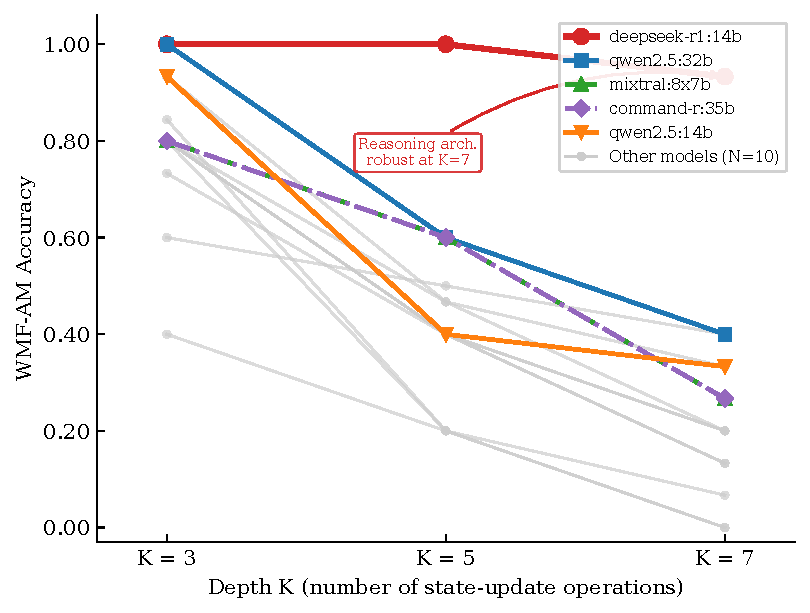
\includegraphics[width=0.72\textwidth]{fig2_depth_profile.pdf}
\caption{\textbf{WMF-AM accuracy by depth $K$ (multi-seed means, $N{=}7$).}
deepseek-r1:14b maintains near-perfect accuracy; others degrade at $K{=}7$.}
\label{fig:depth}
\end{figure}

\section{EMC-lite Results}
\label{app:emclite}

\begin{table}[h]
\centering
\small
\begin{tabular}{lcccccc}
\toprule
Model & F-Det & F-Src & F-Rec & F-Comp & C-Rec & $\Delta$Rec \\
\midrule
qwen2.5:14b     & 0.917 & 0.750 & 0.917 & \textbf{0.917} & 0.972 & $-$0.056 \\
qwen2.5:32b     & 0.917 & 0.750 & 0.917 & \textbf{0.917} & 1.000 & $-$0.083 \\
deepseek-r1:14b & 0.889 & \textbf{0.917} & 0.917 & 0.912 & 1.000 & $-$0.083 \\
llama3.1:8b     & 0.778 & 0.583 & 0.750 & 0.771 & 0.889 & $-$0.139 \\
qwen2.5:7b      & 0.861 & 0.583 & 0.639 & 0.736 & 0.722 & $-$0.083 \\
mistral:7b      & 0.750 & \textbf{0.417} & 0.639 & 0.685 & 0.722 & $-$0.083 \\
gemma2:27b      & 0.861 & 0.583 & 0.528 & 0.667 & 0.611 & $-$0.083 \\
\midrule
$\Delta$ & 0.167 & \textbf{0.500} & 0.389 & \textbf{0.250} & 0.389 & — \\
\bottomrule
\end{tabular}
\caption{\textbf{EMC-lite ($N{=}7$, hardened protocol).}
Source attribution shows strongest differentiation (spread $= 0.500$).}
\label{tab:emclite}
\end{table}

EMC-lite provides preliminary support for the source-conflict slice.
It does not establish EMC as a whole; single-seed evidence only.
$\tau(\text{WMF-AM, EMC-lite}) = 0.250$: substantial independence.

\section{MCC-CE-v2 Results}
\label{app:mccv2}

\begin{table}[h]
\centering
\small
\caption{\textbf{MCC-CE-v2 ($N{=}8$).} Error rates 23--40\% (floor
eliminated); flagging near zero for all models.}
\label{tab:mcc_v2}
\begin{tabular}{lcc|cc}
\toprule
& \multicolumn{2}{c|}{\textbf{Balanced ($n{=}30$)}} & \multicolumn{2}{c}{\textbf{Trap-only ($n{=}20$)}} \\
\textbf{Model} & Error\% & Flag\% & Error\% & Flag\% \\
\midrule
qwen2.5:7b      & 26.7 & 0.0 & 40.0 & 0.0 \\
qwen2.5:14b     & 36.7 & 0.0 & 40.0 & 0.0 \\
qwen2.5:32b     & 30.0 & 0.0 & 25.0 & 0.0 \\
llama3.1:8b     & 26.7 & 0.0 & 40.0 & 0.0 \\
llama3.1:70b    & ---  & --- & 25.0 & 0.0 \\
gemma2:27b      & 30.0 & \textbf{11.1} & 30.0 & 0.0 \\
deepseek-r1:14b & 23.3 & 0.0 & 35.0 & 0.0 \\
mistral:7b      & 30.0 & 0.0 & 40.0 & 0.0 \\
\bottomrule
\end{tabular}
\end{table}

The v1 floor was an artifact of easy questions; v2 models make many
errors but show near-zero self-flagging under the binary protocol.
Alternative designs (continuous confidence, forced ranking) might reveal
partial capacity.

\section{Negative OOD Result}
\label{app:ood}

Two OOD stress-test designs (v1: 5-step NL tasks; v2: $K{=}8$--$9$
interference tasks) produced anti-correlated CEF--OOD relationships
across model pairs. We make no predictive claim. Full assessment requires
$N \geq 11$ with process-sensitive downstream tasks.

\section{Full Validity Analyses}
\label{app:validity}

The validity summary table appears in the main text
(Table~\ref{tab:validity}). Below we provide additional details.

\paragraph{Convergent validity details.}
AGENT-PQ: 10 multi-step scenarios scored by LLM judge (GPT-4o) on
4 rubric dimensions. CONV-RFPOC: 15 reasoning problems with
counterfactual chain perturbation. RFPOC $= 1 - P(\text{same answer}
\mid \text{perturbed chain})$. Full protocol in
Appendix~\ref{app:agentpq}.
\textbf{Limitation:} LLM judge may introduce shared bias.

\paragraph{Construct separation (WMF-AM $\leftrightarrow$ CLA-DC).}
$\tau = 0.905$: no evidence of separability at $N{=}7$. Both involve
state tracking under load. Planned discriminant test at $N \geq 15$.
CLA-CR-v3 provides a structurally independent CLA measure.
Even if CLA-DC merges with WMF-AM, WMF-AM, MCC-MA, and EMC-lite
remain separable ($\tau \leq 0.250$).

\paragraph{Sensitivity.}
LOMO for CONV-RFPOC vs AGENT-PQ: $\tau$ ranges 0.600--1.000
(mean 0.833). Leave-one-family-out (Qwen, $N{=}4$): $\tau = 0.667$.
After Holm correction, RFPOC--AGENT-PQ remains significant
($p_\text{adj} = 0.021$).

\paragraph{Multiple testing.}
Three primary hypotheses; all others exploratory.

\paragraph{Benchmark governance.}
All headline results use frozen protocol versions. Probe revisions were
motivated by floor/ceiling effects, not model-specific tuning.

\section{AGENT-PQ Evaluation Protocol}
\label{app:agentpq}

\textbf{AGENT-PQ} uses 10 multi-step scenarios where each model operates
within a tool-use scaffold. A separate LLM judge (GPT-4o, temperature
$= 0$) scores each trajectory on four rubric dimensions:
plan coherence, state tracking, error recovery, goal adherence.
AGENT-PQ $= \text{mean of 4 rubric scores} / 4$.
AGENT-TC is the binary success rate on the same scenarios.

\textbf{CONV-RFPOC} administers 15 reasoning problems with
counterfactual chain perturbation.
RFPOC $= 1 - P(\text{same answer} \mid \text{perturbed chain})$.

\section{Complete Experimental Protocols}
\label{app:protocols}

Full prompt templates, parameter specifications, scoring procedures, and
reference implementations for all 11 sub-dimensions are provided in the
supplementary materials.

\section{Weight Sensitivity Analysis}
\label{app:weights}

Three weighting schemes (proposed, equal, PCA-derived) are evaluated.
Per-dimension profiles are primary; composites are exploratory only.

\section{Dissociation Case Studies}
\label{app:dissociation}

Matched dissociation pairs: deepseek-r1:14b and qwen2.5:14b share
similar EMC-lite (0.912 vs.\ 0.917) but differ on WMF-AM (0.983 vs.\
0.467). mistral:7b and llama3.1:8b have similar WMF-AM but differ on
EMC-lite. These cross-dimension pairs anchor the multiple realizability
argument.

\section{Worked Example: WMF-AM at Depth $K{=}3$}
\label{app:worked}

\noindent\textbf{Setup.} ``A warehouse has 3~items: Widget=50,
Gadget=30, Sprocket=20.'' Three updates: ``Ship 10~Widgets,''
``Receive 25~Gadgets,'' ``Transfer 5~Sprockets to overflow.''

\noindent\textbf{Correct.} Widget=40, Gadget=55, Sprocket=15.

\noindent\textbf{Scoring.} Exact match per item. deepseek-r1:14b scores
1.000 at $K{=}7$; llama3.1:8b scores 0.050. Both score 0.90--0.95 on
outcome correctness. This is the Completion Fallacy in action.

\section{Novelty Classification}
\label{app:novelty}

\begin{table}[h]
\centering
\small
\caption{Novelty tier for all 11 sub-dimensions. Tier 1 = novel;
Tier 2 = novel reframing.}
\label{tab:novelty}
\begin{tabular}{llp{6.5cm}}
\toprule
\textbf{Sub-dim} & \textbf{Tier} & \textbf{Prior art / differentiation} \\
\midrule
WMF-AM & 1 & Entity Tracking~\citep{entitytracking2023}: passive retrieval; WMF-AM = sequential transformation \\
WMF-IM & 2 & Wang \& Sun~\citep{wang2025unableforgetproactiveinterference}: key-value pairs; WMF-IM = NL multi-turn \\
WMF-IR & 2 & Extended to domain-varied materials \\
MCC-MA & 1 & Gnosis~\citep{ghasemabadi2025can} requires internals; MCC-MA = prompting only \\
MCC-CE & 1 & Reflexion~\citep{shinn2023reflexion}: aggregate; MCC-CE decomposes detection/correction \\
EMC-TO & 1 & No prior LLM temporal ordering measurement \\
EMC-EI & 1 & No prior cross-episode interference diagnostic \\
EMC-SA & 2 & Interference-conditioned attribution \\
CLA-DC & 1 & Intell.\ Degradation~\citep{wang2026intelligence}: magnitude; CLA-DC = shape \\
CLA-RA & 1 & Not previously measured \\
CLA-CR & 1 & Not previously measured \\
\bottomrule
\end{tabular}
\end{table}

\end{document}
